\documentclass[twocolumn,preprintnumbers,amsmath,amssymb,longbibliography]{revtex4-1}

\usepackage{graphicx}% Include figure files
\usepackage{dcolumn}% Align table columns on decimal point
\usepackage{bm}% bold math
\usepackage{float}
\usepackage{siunitx}

% Set one inch margins all around
\setlength\textwidth{6.5in}
\setlength\oddsidemargin{0in}
\setlength\evensidemargin{0in}

\setlength\textheight{9in}
\setlength\topmargin{-0.25in}
\setlength\headheight{0in}

\begin{document}

\title{Viability of Playing Music with Rubber Bands}% Force line breaks with \\

\author{Aether Zhou}
\affiliation{%
Department of Physics, University of California, Santa Barbara, CA 93106
}%

\date{\today}% It is always \today, today

\begin{abstract}
    Rubber bands are commonly used our daily life, because of its good quality of elasticity and cheap price. When tensions are applied to stretch a rubber band, it exhibits some characteristics of strings used in instruments. And the frequency generated from a commonly accessible rubber band in the markets covers four octaves, which made the rubber bands possible to be used to play multiple kinds of music. However, rubber bands are easily deformed and broken due to their low stiffness, which can lead to short life-time and more works in tuning. Hence, common rubber bands in the markets are not suitable to play music. 
\end{abstract}

\maketitle

\section{Introduction}
    Similar to strings, a vibrating rubber band has small amplitudes relative to the length of the band, which allows us to approximate the wave behavior on a stretched rubber band as that on a stretched string.\\\\
    For a stretched string, the standing wave on it has the following relation to the length of it and tension applied\cite{freq}:
    \begin{eqnarray}
        f=\frac{\sqrt{T/\lambda}}{2L} \label{wave}\, ,
    \end{eqnarray}
    where $f$ stands for the frequency, $T$ is tension, $\lambda$ is mass density and $L$ is total length of the string.
    \\
    \\
    From Eq.~\eqref{wave}, we can obtain the dependency of frequency on tension and on wavelength respectively:
    \begin{eqnarray}
        f\propto \sqrt{T}\label{ten}\,,
    \end{eqnarray}
    and
    \begin{eqnarray}
        f\propto \frac{1}{L}\label{len}\, .
    \end{eqnarray}
    \\
    Hence, we are allowed to discover the range for the frequency of vibrating rubber bands and to see either the pitch coverage is enough to play most music or not. And from there we could discuss the appropriateness of building an instrument with rubber bands. 
    \\
\section{Experimental Methods}
    The experiment setup contains a spring scale, a large box, several screws, and rubber bands. Screws are used to fix rubber bands to different length under different forces applied; and they are also used to create nodes on the stretched bands, so the wavelength of standing waves on the rubber bands can be changed in a certain range. Hence, a structure in Fig.~\ref{rubber} is built, which is similar to strings on an instrument called ``guzheng".
\begin{figure}[H]
\centering
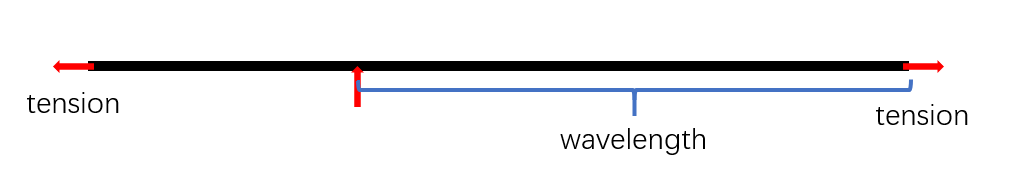
\includegraphics[width=8cm]{rubber.png}
\caption{\label{rubber} Setup of the vibrating rubber band.} 
\end{figure}
    \\
    \\
    Also, the spring scale used can measure forces between $0$ and $10$ Newton, with uncertainty of $0.2\si{.N}$. The ruler used to measure rubber band's length and the wavelength can measure lengths ranging from $0$ to $100$ centimeters, with uncertainty of $0.1 \si{.cm}$. The rubber bands used in this experiment have diameter of about $4.10 \si{.cm}$ before being stretched, and the diameter increases after each stretching. After being stretched under tension of $10\si{.N}$ for several seconds and released for more than five times, the rubber band's diameter will stabilize around $4.60\si{.cm}$. The cross-section area of rubber bands  used is about $4.0\si{.mm^2}$. The elastic characteristic of the rubber bands used are shown in Fig.~\ref{hook}.
\begin{figure}[H]
\centering
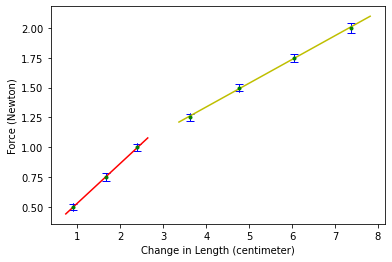
\includegraphics[width=8cm]{hook.png}
\caption{\label{hook} Force-length relation of the rubber bands used.} 
\end{figure}
    The data are fitted by linear relation between tension and change in length of rubber bands, and the rubber bands used in this experiment tend to break under tension larger than $10\si{.N}$ or being stretched to longer than $50\si{.cm}$.
    \\
    \\
    And the frequency data is measured by a smartphone app called ``phyphox''. 
    Under these setup, several measurements are made to check the wavelength-frequency and tension-frequency relations of a stretched string. 

\section{Results}
The following is the measurement of frequency for various wavelength under fixed tension of $10\si{.N}$. And the data is fitted by the wavelength-frequency relation given by Eq.~\eqref{len}.
\begin{figure}[H]
\centering
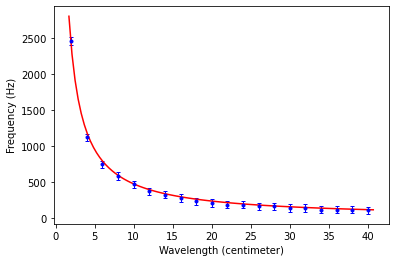
\includegraphics[width=8cm]{l-f.png}
\caption{\label{sp} Wavelength-frequency relation under fixed tension of $10 \si{.N}$.} 
\end{figure}
From these measurement we can conclude that the rubber band used can generate sound of frequency between $200\si{.Hz}$ and $2000\si{.Hz}$ when being set to proper wavelength. And the frequency coverage is about three octaves in music.\cite{freqTable} Hence, the pitch coverage of the rubber band is suitable to play many simple music.
\\
\\
Besides the pitch coverage, the frequency generated under various tension exerted is also important for an instrument. This is because the frequency-tension relation is involved in the tuning process, which is necessary before each time of playing. And the following is the measurement  of tension-frequency relation for fixed wavelength of $8\si{.cm}$. The data is fitted by Eq.~\eqref{ten}.
\begin{figure}[H]
\centering
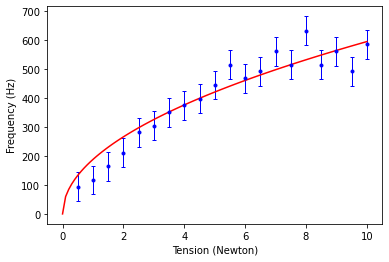
\includegraphics[width=8cm]{t-f.png}
\caption{\label{sp} Tension-frequency relation for fixed wavelength of $8\si{.cm}$} 
\end{figure}
From this we can see that the frequency increase with tension is stable under small tension (less than $5\si{.N}$), and the data does not meet the expected value for large tension (around $9\si{.N}$). This is possibly due to deformation of the rubber band after several times of stretching. 

\section{Analysis} 
The deformation of the rubber bands is a possible obstacle to prevent rubber being used in instrument. The following measurement reflects the effect of deformation on the rubber bands. 
\begin{figure}[H]
\centering
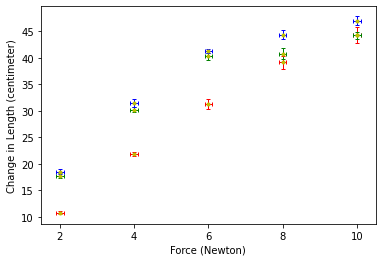
\includegraphics[width=8cm]{deform.png}
\caption{\label{deform} Tension-length relation of the rubber bands. Red data is for the first stretching of rubber bands. Green data is for the second time stretch and blue data for the third time.} 
\end{figure}
As measured, the rubber bands become easier to be stretched after being stretched for several times. And one factor leads to this is the fissure on the rubber bands.
\begin{figure}[H]
\centering
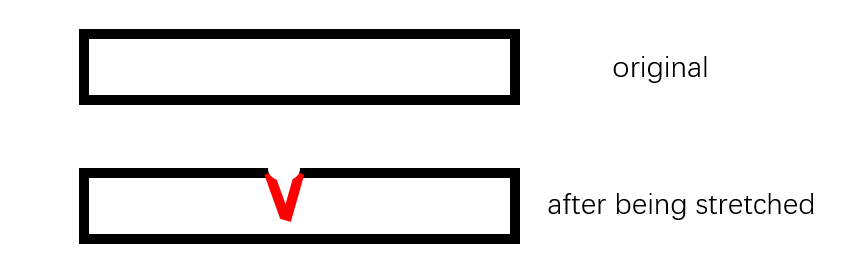
\includegraphics[width=8cm]{cleave.png}
\caption{\label{slit} Magnified view of rubber bands.} 
\end{figure}
As shown in Fig.~\ref{slit}, many fissures appear on the rubber band after it is being stretched. Hence, the cross-section area near the fissures are smaller than the original, which means the stress exerted around that region is larger under the same tension. As a result, the rubber bands can extend longer under the same force exerted. \\
\\
However, as the fissures accumulate, the rubber bands tend to break more easily.

\section{Conclusions}
In conclusion, rubber bands are not suitable for music playing. Although it can cover many pitches, the trouble with tuning and low quality after multiple stretching makes the rubber band unsuitable for long time use. 

\begin{acknowledgments}
Thanks to Dr. Jayich for guidance of this lab and editing of this report.

\end{acknowledgments}


\bibliography{references}% Produces the bibliography via BibTeX.

\end{document}
%
% ****** End of file apssamp.tex ******
